\documentclass[10pt]{article}
\usepackage[margin=1in]{geometry}
 \usepackage{auto-pst-pdf}
\usepackage{graphicx}
%\usepackage{arydshln}
\usepackage{ifpdf}
\ifpdf
  \usepackage{epstopdf}
\fi
\usepackage{multirow}
\usepackage{epsfig}
\usepackage{float}
\usepackage{url}
\usepackage{color}
\usepackage{subfigure}

%\newcommand\solidrule[1][1cm]{\rule[0.5ex]{#1}{.4pt}}
%\newcommand\dashedrule{\mbox{%
%  \solidrule[2mm]\hspace{2mm}\solidrule[2mm]\hspace{2mm}\solidrule[2mm]}}
  
%\usepackage{hyperref}

\begin{document}
\title{A Study of INC Runs in Sequence}

\author{
Young-Kyoon Suh\\
}
\maketitle

\section{Description}
In this document we discuss characteristics of INC runs in sequence. 

There are two big subjects included in the document.
Specifically, the first subject relates running a series of INCs in a batch, pausing the run, and then resuming 
the run, rather than repeating the same INC multiple times. 
That is, INC1, ..., INC16384 are consecutively run as a batch, and 
then the entire batch run sleeps for an hour, and then 
another batch run of INC1, ..., INC16384 begins, stops, and resumes, and so forth.

The second subject concerns breaking up 
a whole run of 1000 samples into 200 samples, thereby yielding five different histograms. 

\subsection{Experiment Notes}
Table~\ref{tab:exp_notes} provides a short description of our experimental runs, 
on which the following histograms are based.

%% done
\begin{table}[h]
\begin{center}
\begin{tabular}{|p{2cm}|p{3cm}|p{6cm}|p{4cm}|} \hline
Machine & Task Length (sec) & Description & Experiment Period\\ \hline
{\tt sodb9} &  INC16 & Each run with 1,000 samples & 2017-03-02 $\sim$ 2017-03-07\\ \hline
{\tt sodb9} &  INC1~INC16384 & One run in which each INC has 30 samples & 2018-11-17 $\sim$ 2018-12-02\\ \hline
\end{tabular}
\end{center}
\vspace{-.2in}
\caption{Notes on experiment runs used for histograms\label{tab:exp_notes}}
\end{table}

\newpage
\section{INC Run in Sequence}

\begin{figure}[hp!]
	\centering
	\subfigure[PT frequency on INC1 on {\tt sodb9}]{
		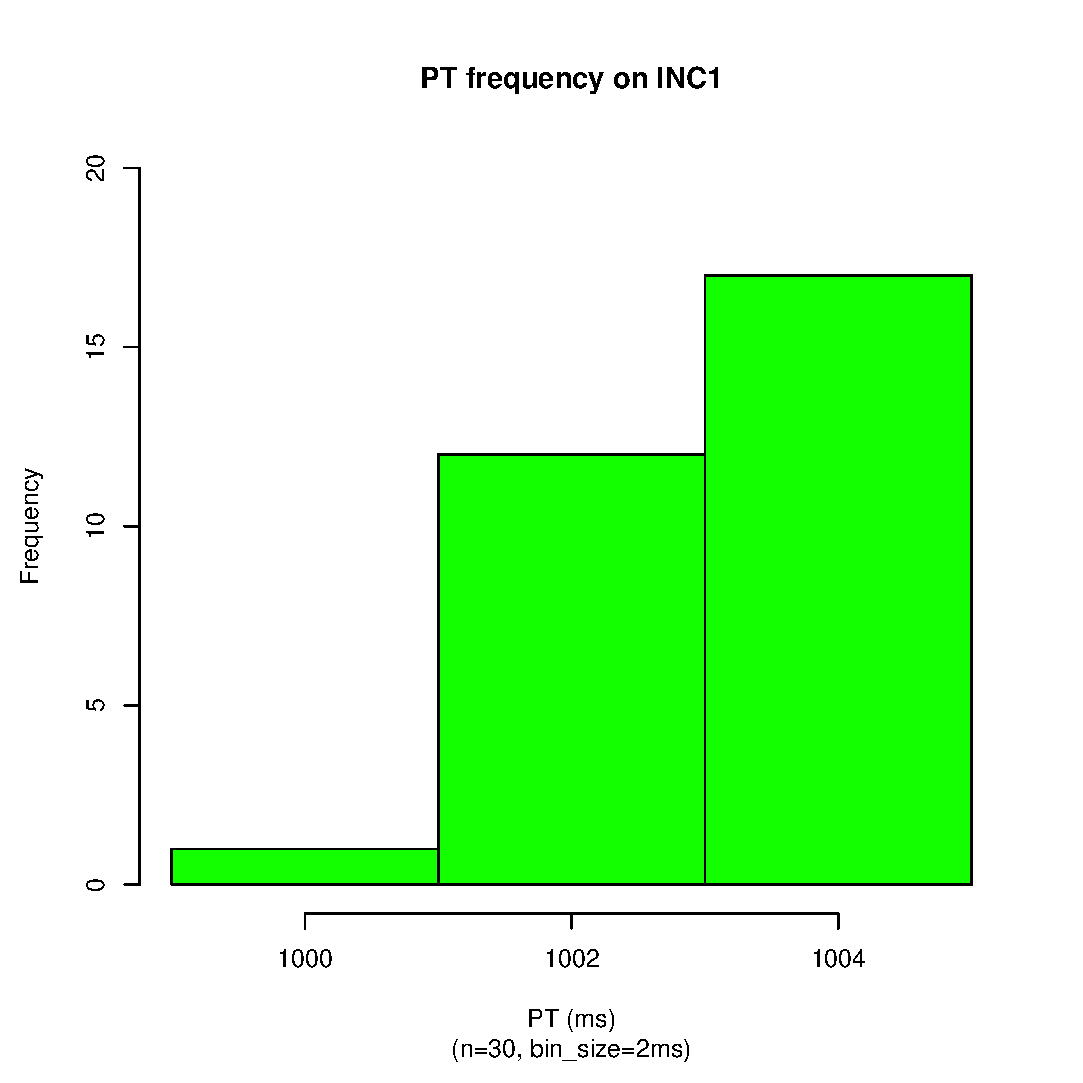
\includegraphics[scale=0.43]{1_sec_pt_hist.eps}
		\label{fig:inc1}
	}
	\subfigure[PT frequency on INC2 on {\tt sodb9}]{
		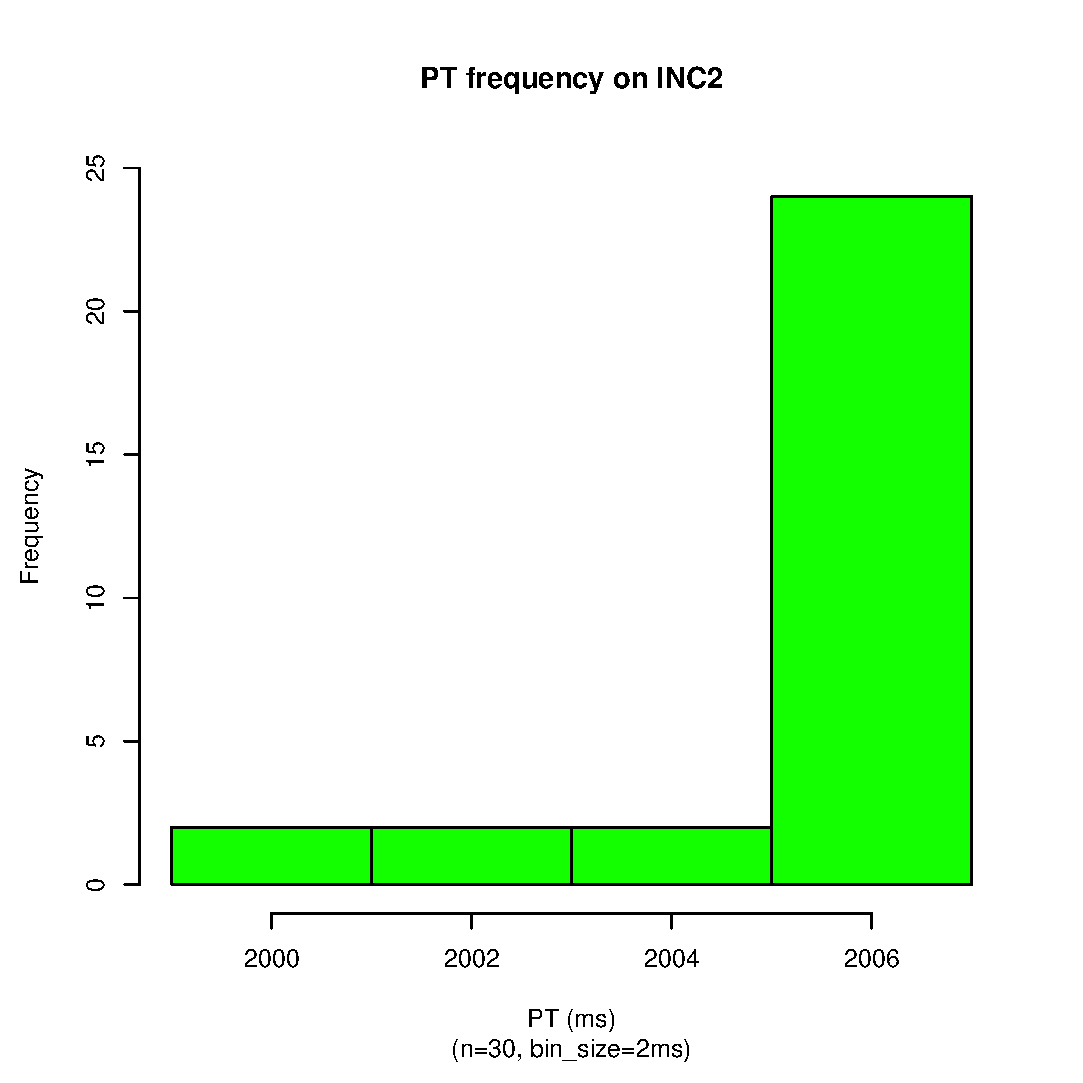
\includegraphics[scale=0.43]{2_sec_pt_hist.eps}
		\label{fig:inc2}
	}
	\subfigure[PT frequency on INC4 on {\tt sodb9}]{
		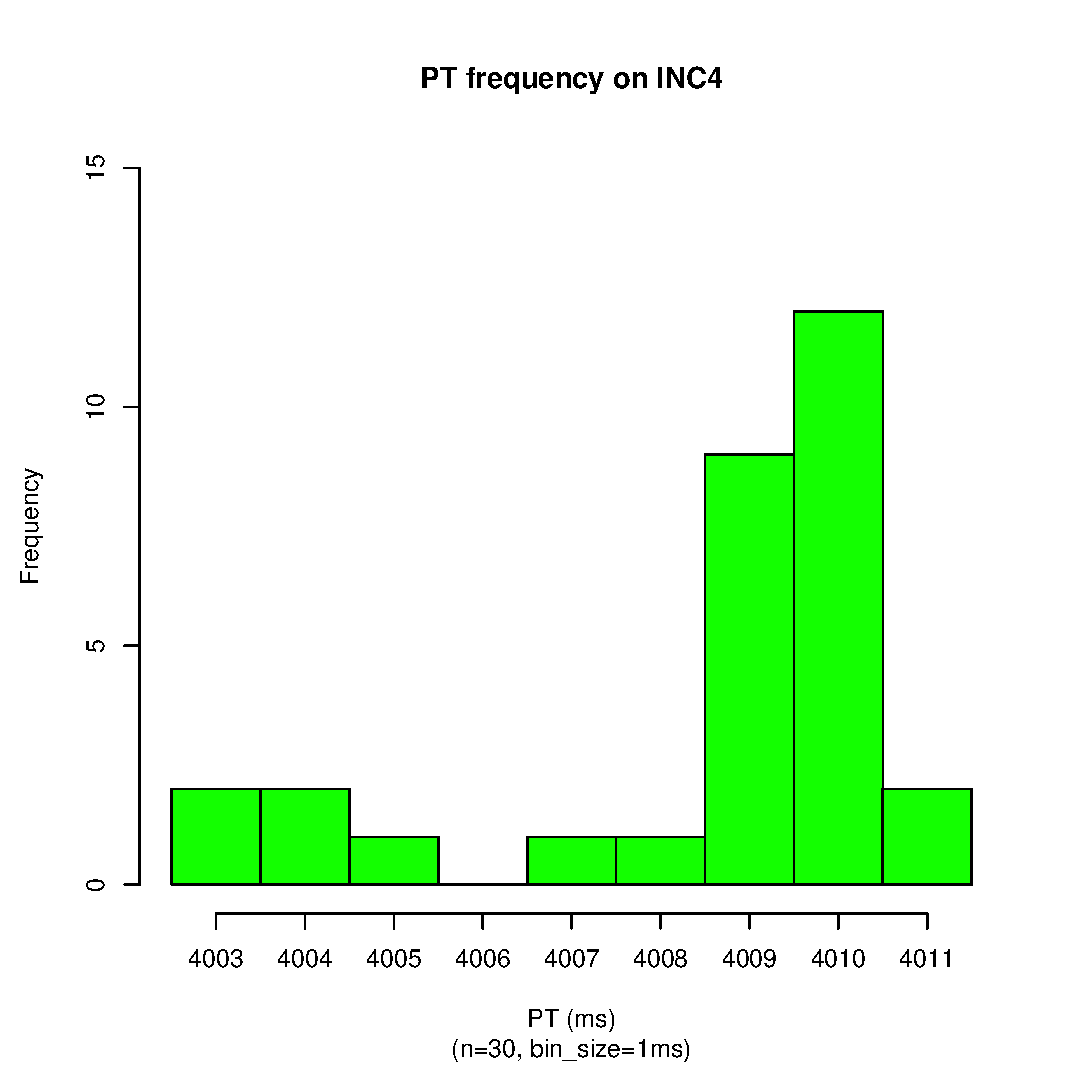
\includegraphics[scale=0.43]{4_sec_pt_hist.eps}
		\label{fig:inc4}
	}
	\subfigure[PT frequency on INC8 on {\tt sodb9}]{
		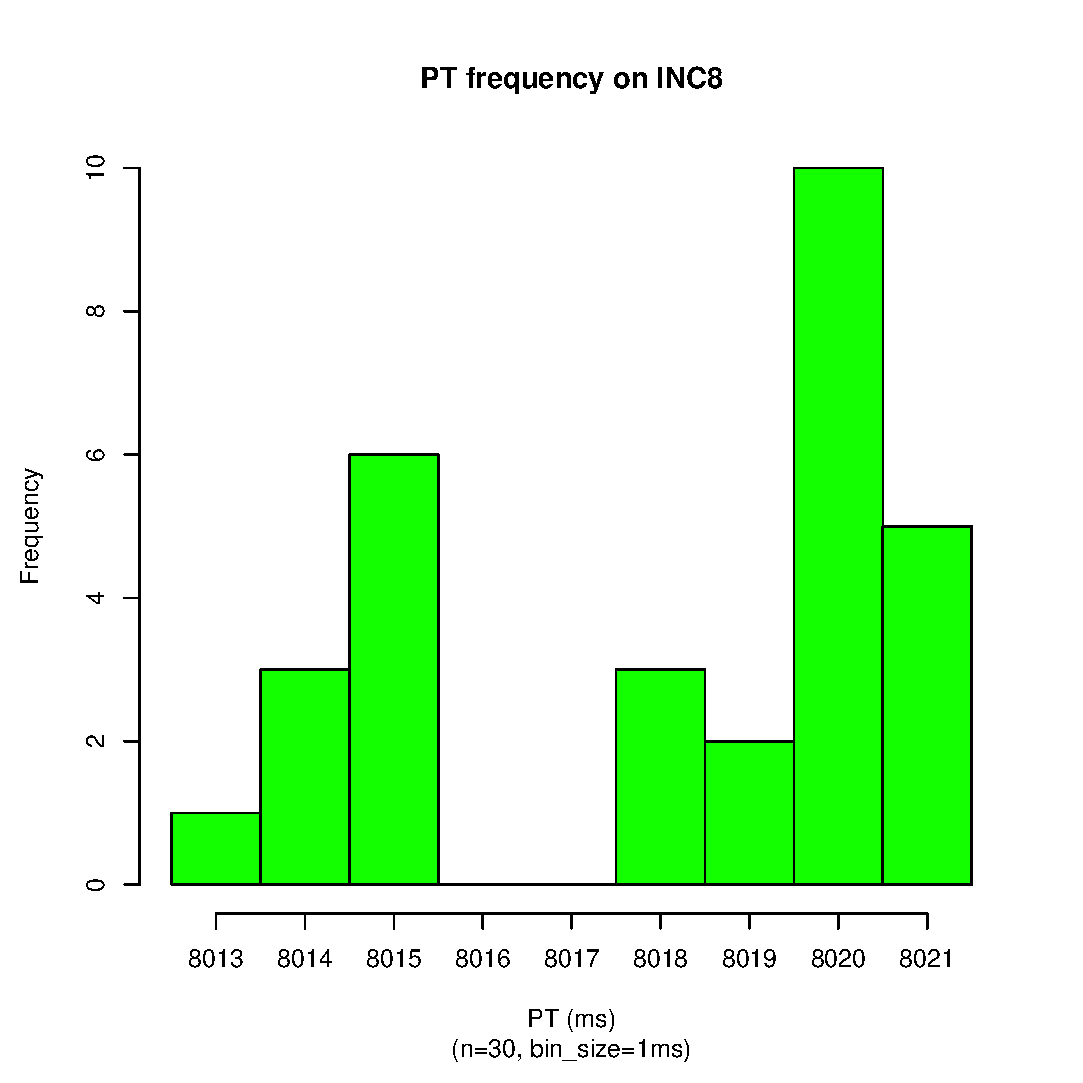
\includegraphics[scale=0.43]{8_sec_pt_hist.eps}
		\label{fig:inc8}
	}
	\caption{PT Histograms of INC1 ... INC8~\label{fig:s9_r2_pt_hist1}}
\end{figure}

\begin{figure}[hp!]
	\centering
	\subfigure[PT frequency on INC16 on {\tt sodb9}]{
		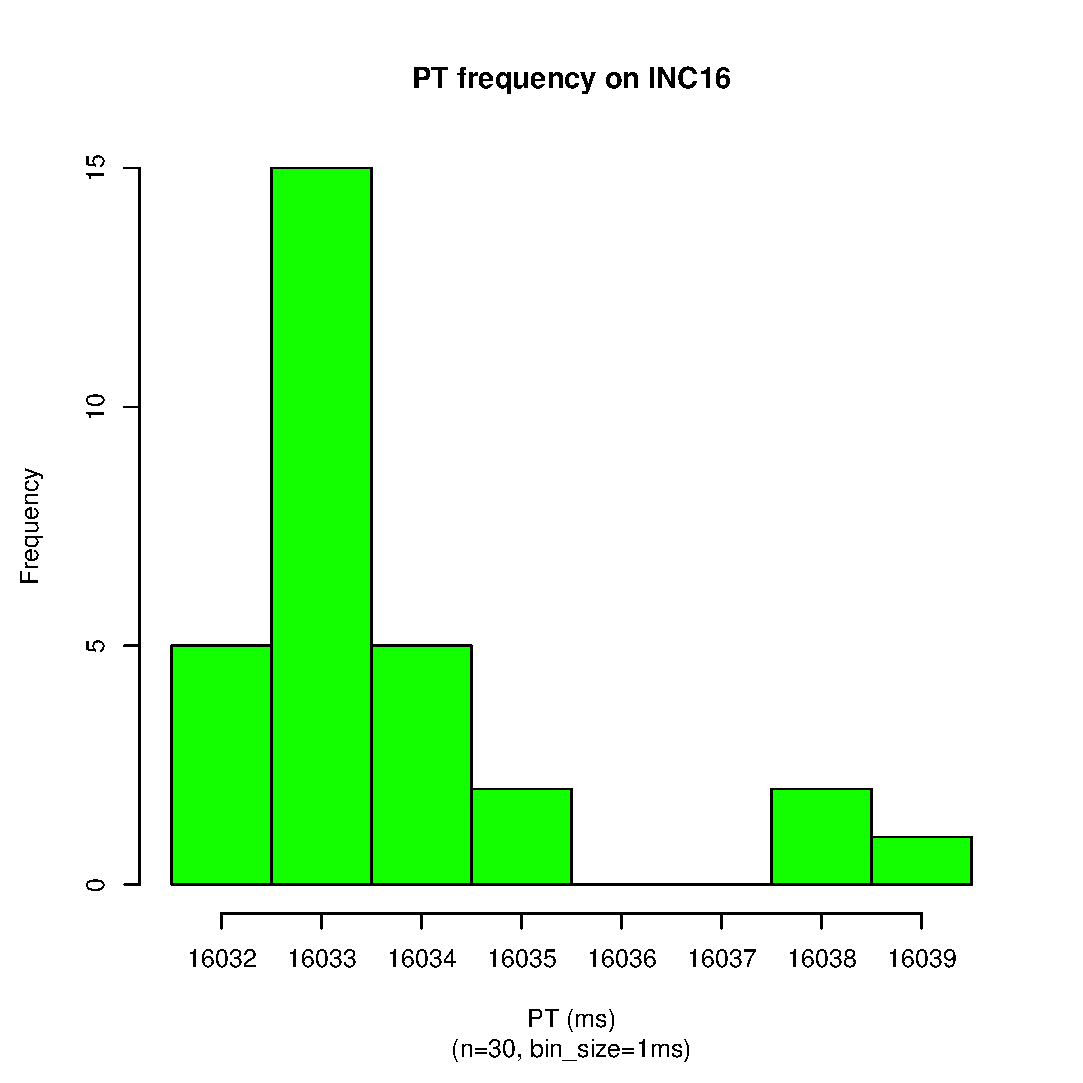
\includegraphics[scale=0.43]{16_sec_pt_hist.eps}
		\label{fig:inc16}
	}
	\subfigure[PT frequency on INC32 on {\tt sodb9}]{
		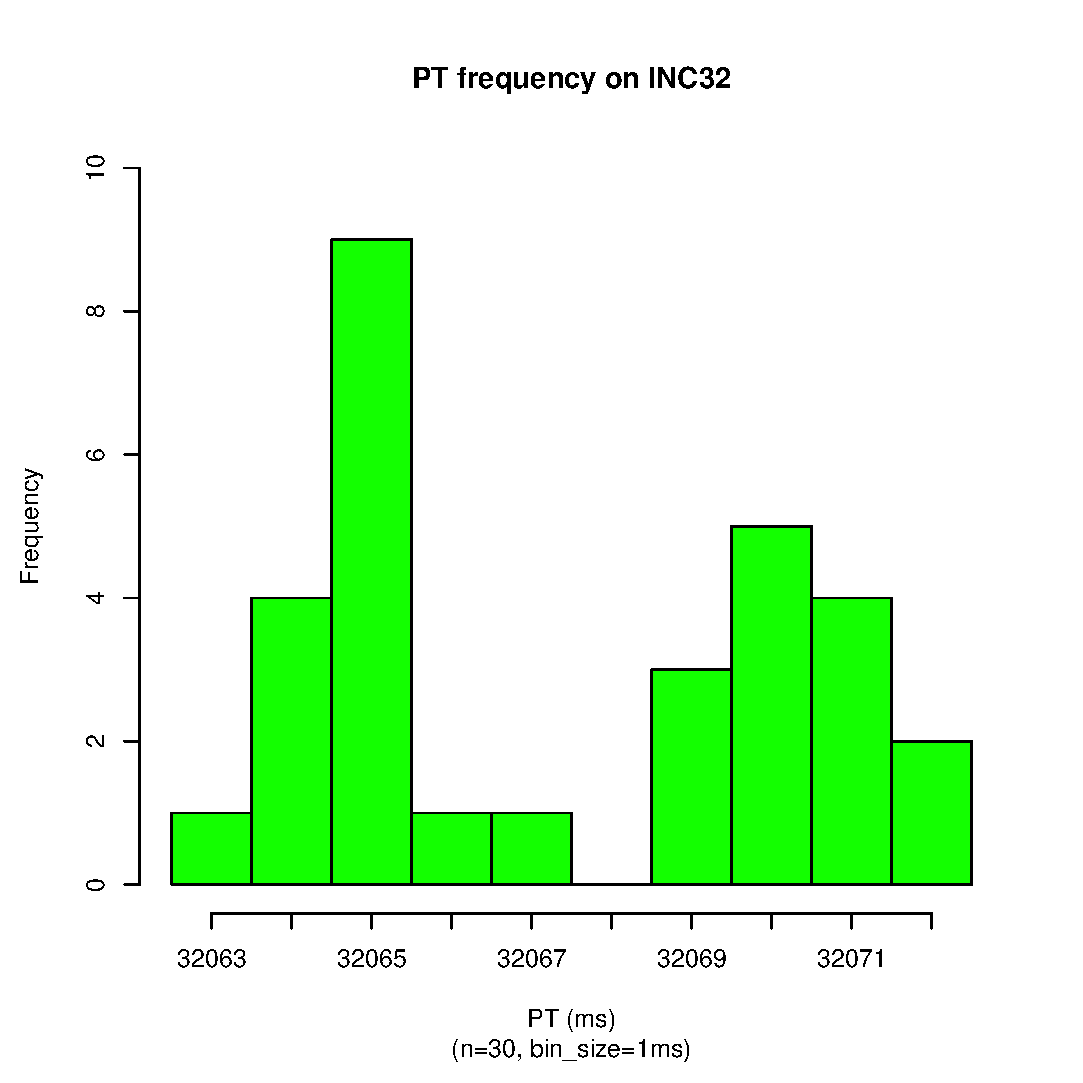
\includegraphics[scale=0.43]{32_sec_pt_hist.eps}
		\label{fig:inc32}
	}
	\subfigure[PT frequency on INC64 on {\tt sodb9}]{
		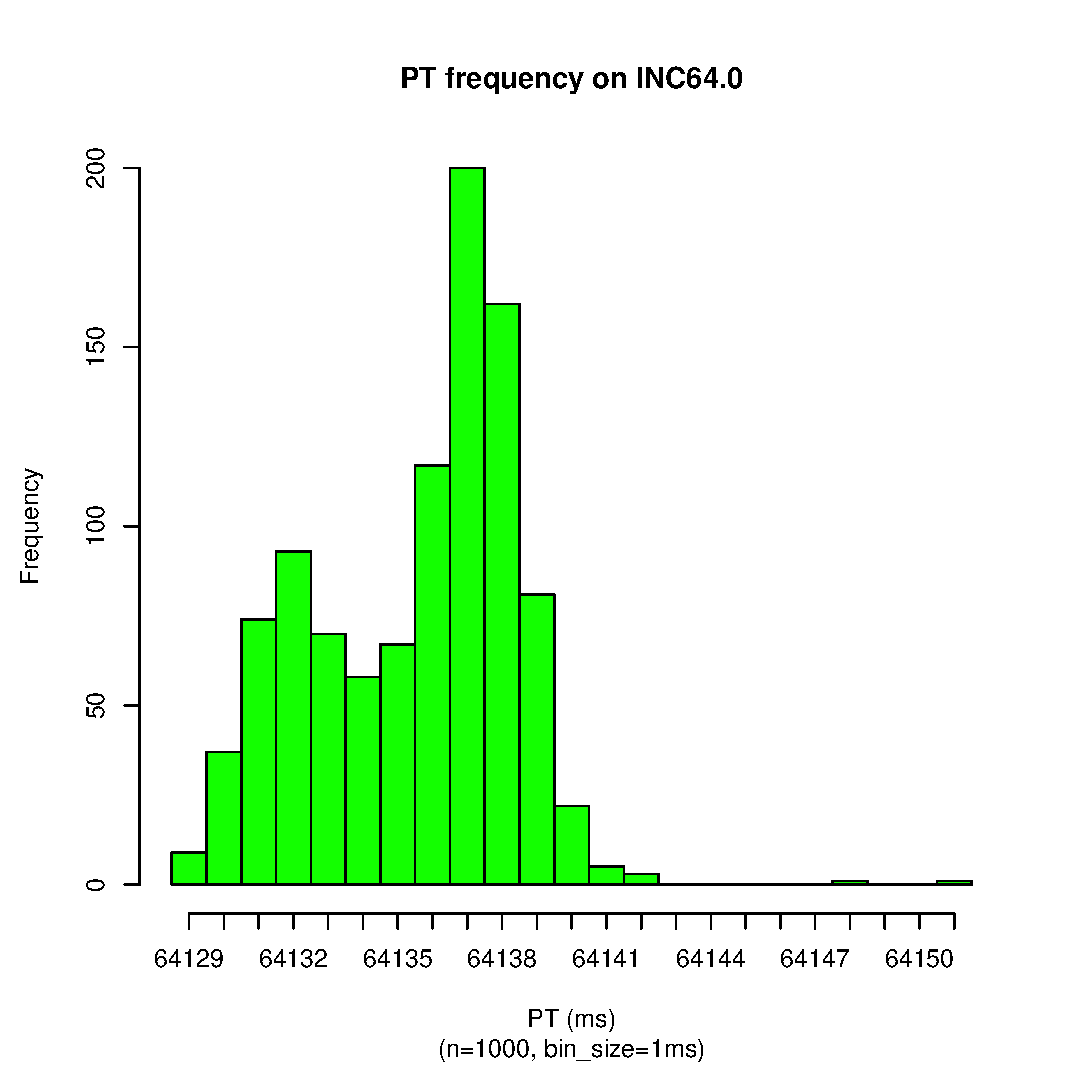
\includegraphics[scale=0.43]{64_sec_pt_hist.eps}
		\label{fig:inc64}
	}
	\caption{PT Histograms of INC16 ... INC64\label{fig:s9_r2_pt_hist2}}
\end{figure}

\begin{figure}[hp!]
	\centering
	\subfigure[PT frequency on INC128 on {\tt sodb9}]{
		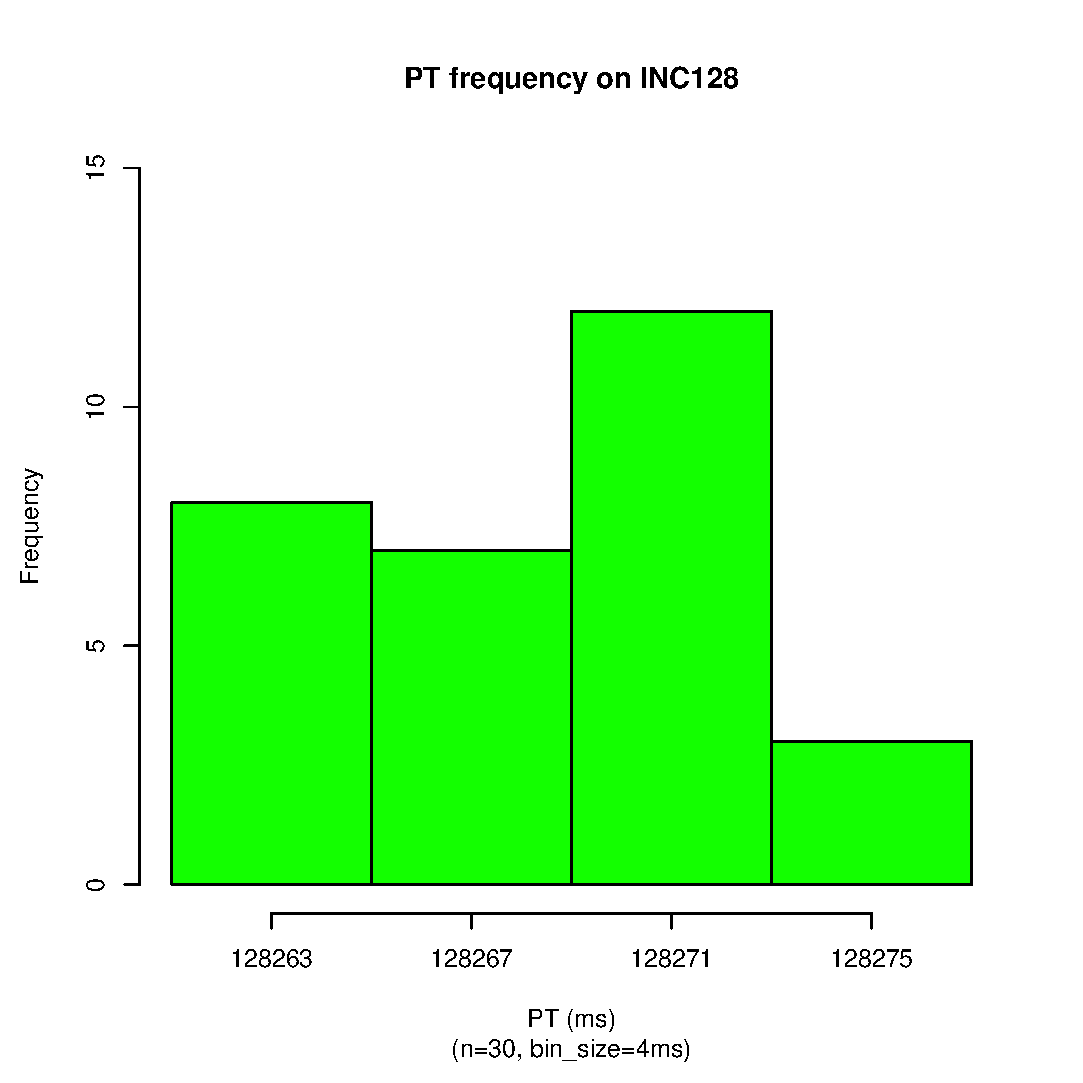
\includegraphics[scale=0.43]{128_sec_pt_hist.eps}
		\label{fig:inc128}
	}
	\subfigure[PT frequency on INC256 on {\tt sodb9}]{
		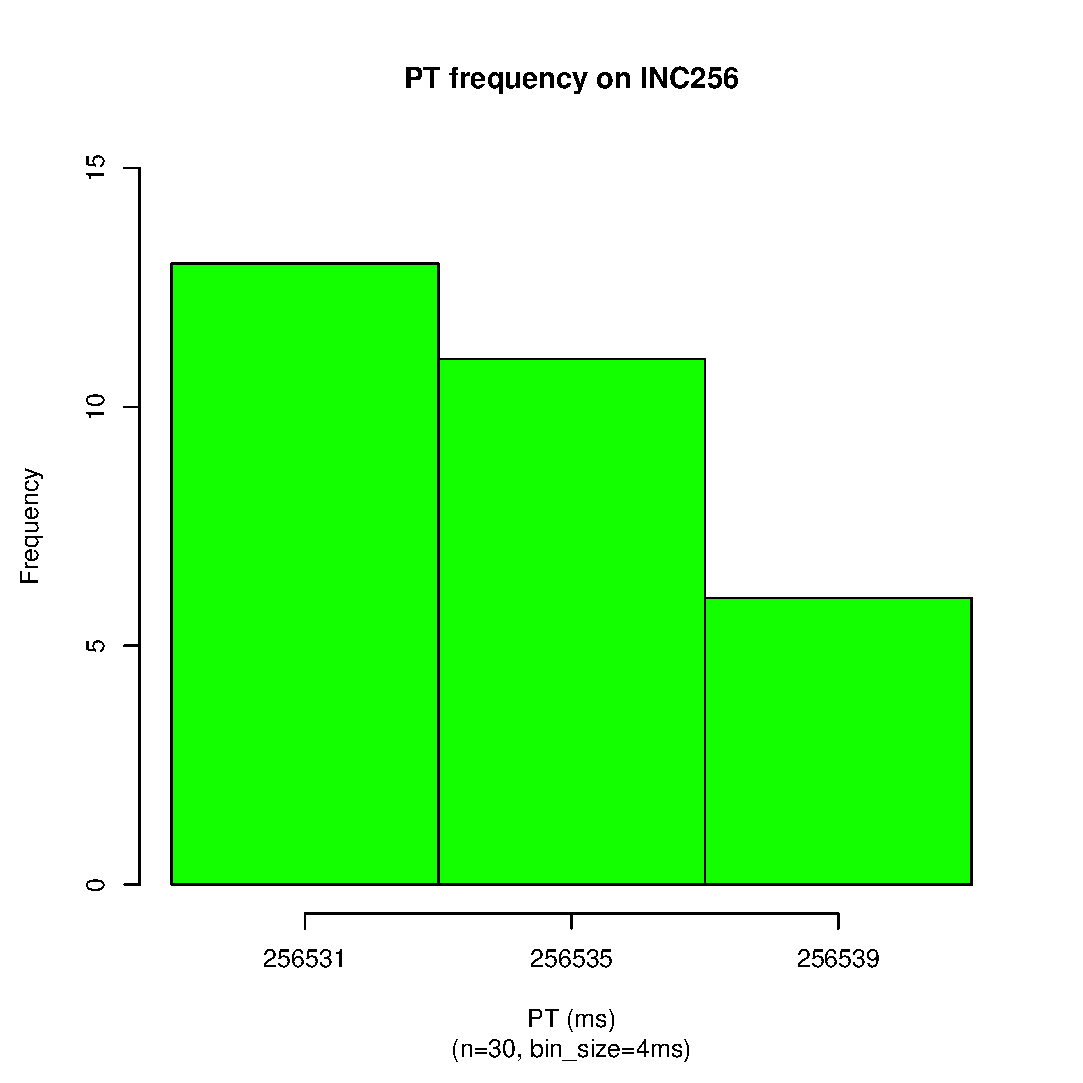
\includegraphics[scale=0.43]{256_sec_pt_hist.eps}
		\label{fig:inc256}
	}
	\subfigure[PT frequency on INC512 on {\tt sodb9}]{
		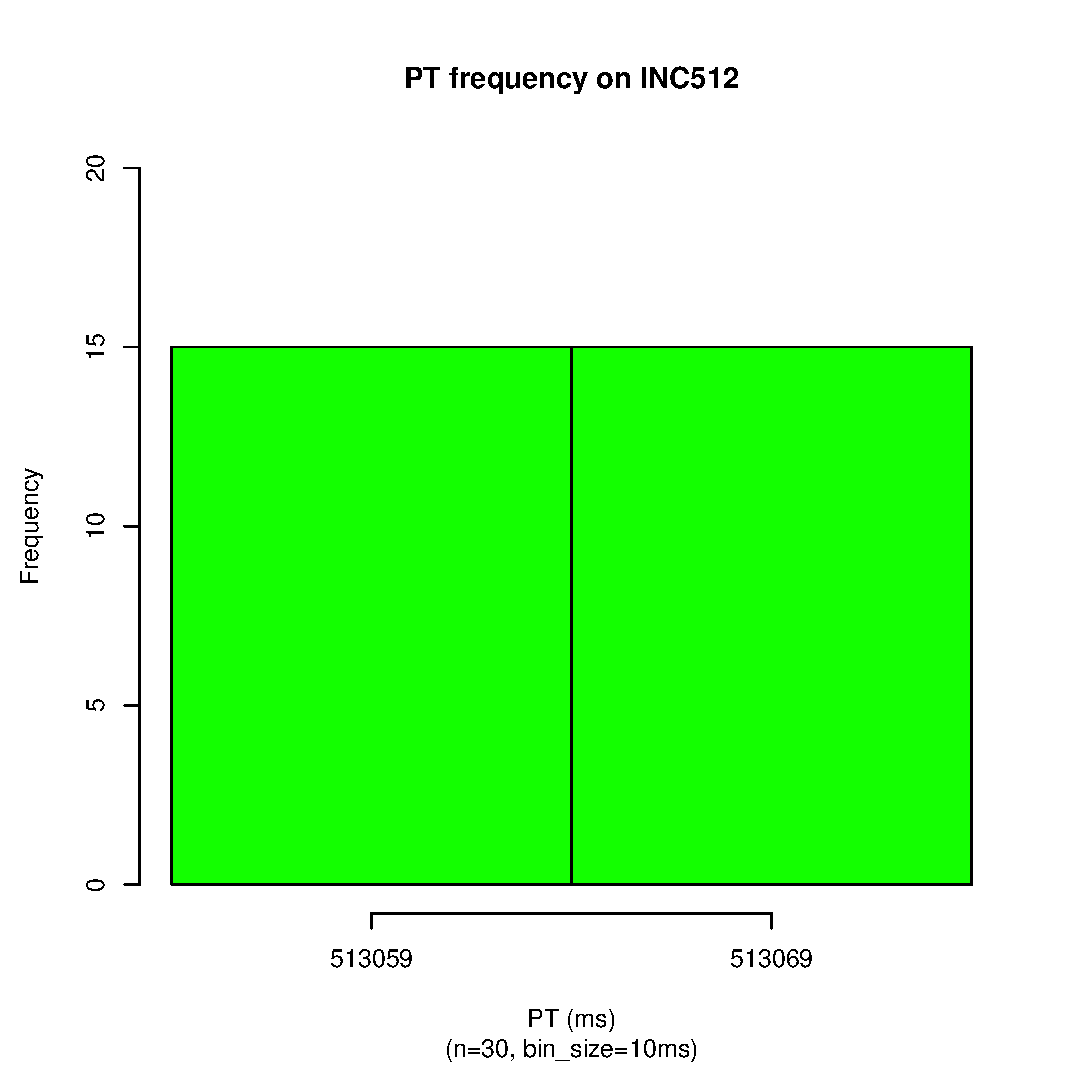
\includegraphics[scale=0.43]{512_sec_pt_hist.eps}
		\label{fig:inc512}
	}
	\subfigure[PT frequency on INC1024 on {\tt sodb9}]{
		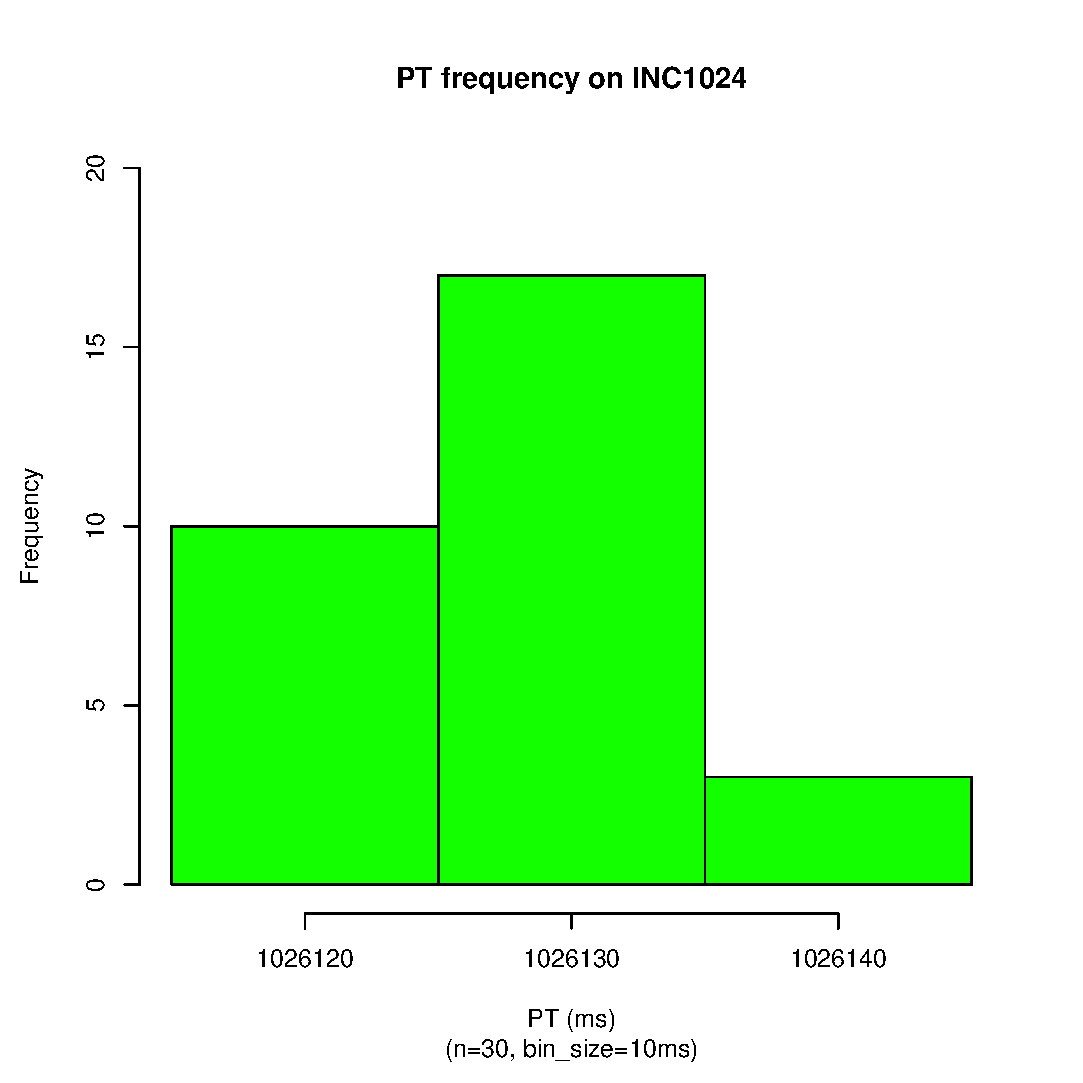
\includegraphics[scale=0.43]{1024_sec_pt_hist.eps}
		\label{fig:inc1024}
	}
	\caption{PT Histograms of INC256 ... INC1024~\label{fig:s9_r2_pt_hist3}}
\end{figure}

\begin{figure}[t]
	\centering
	\subfigure[PT frequency on INC2048 on {\tt sodb10}]{
		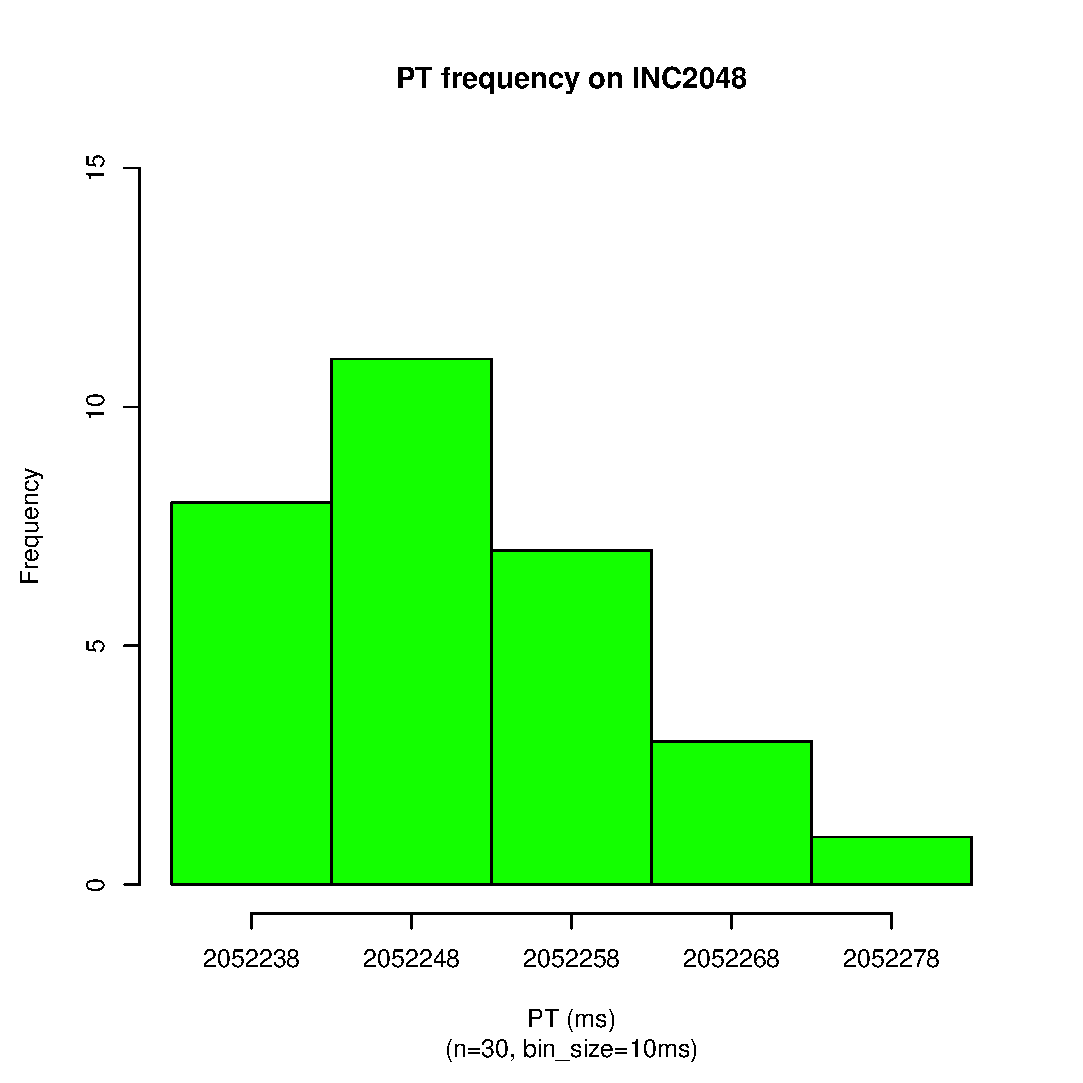
\includegraphics[scale=0.43]{2048_sec_pt_hist.eps}
		\label{fig:inc2048}
	}
	\subfigure[PT frequency on INC4096 on {\tt sodb12}]{
		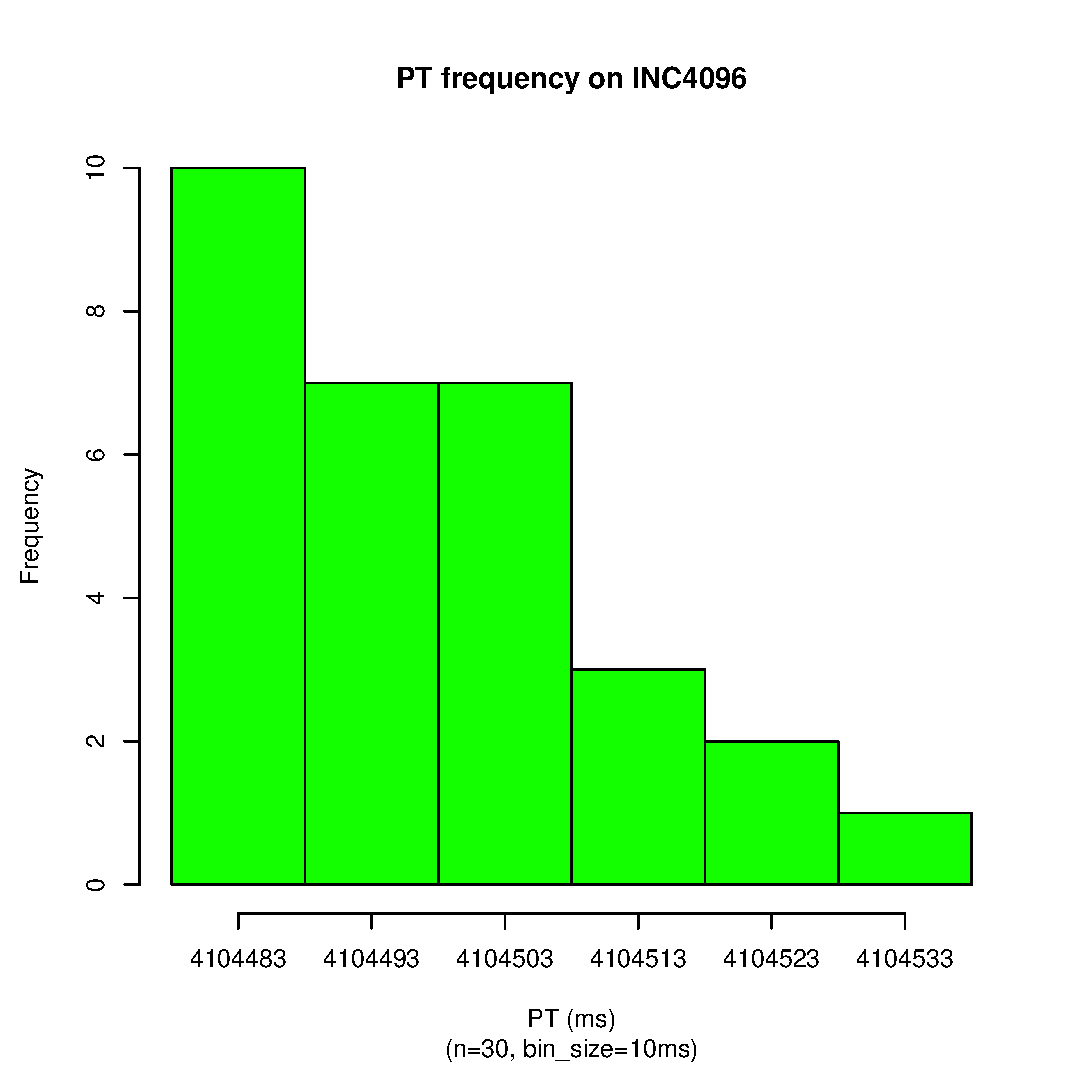
\includegraphics[scale=0.43]{4096_sec_pt_hist.eps}
		\label{fig:inc4096}
	}
	\subfigure[PT frequency on INC8192 on {\tt sodb10}]{
		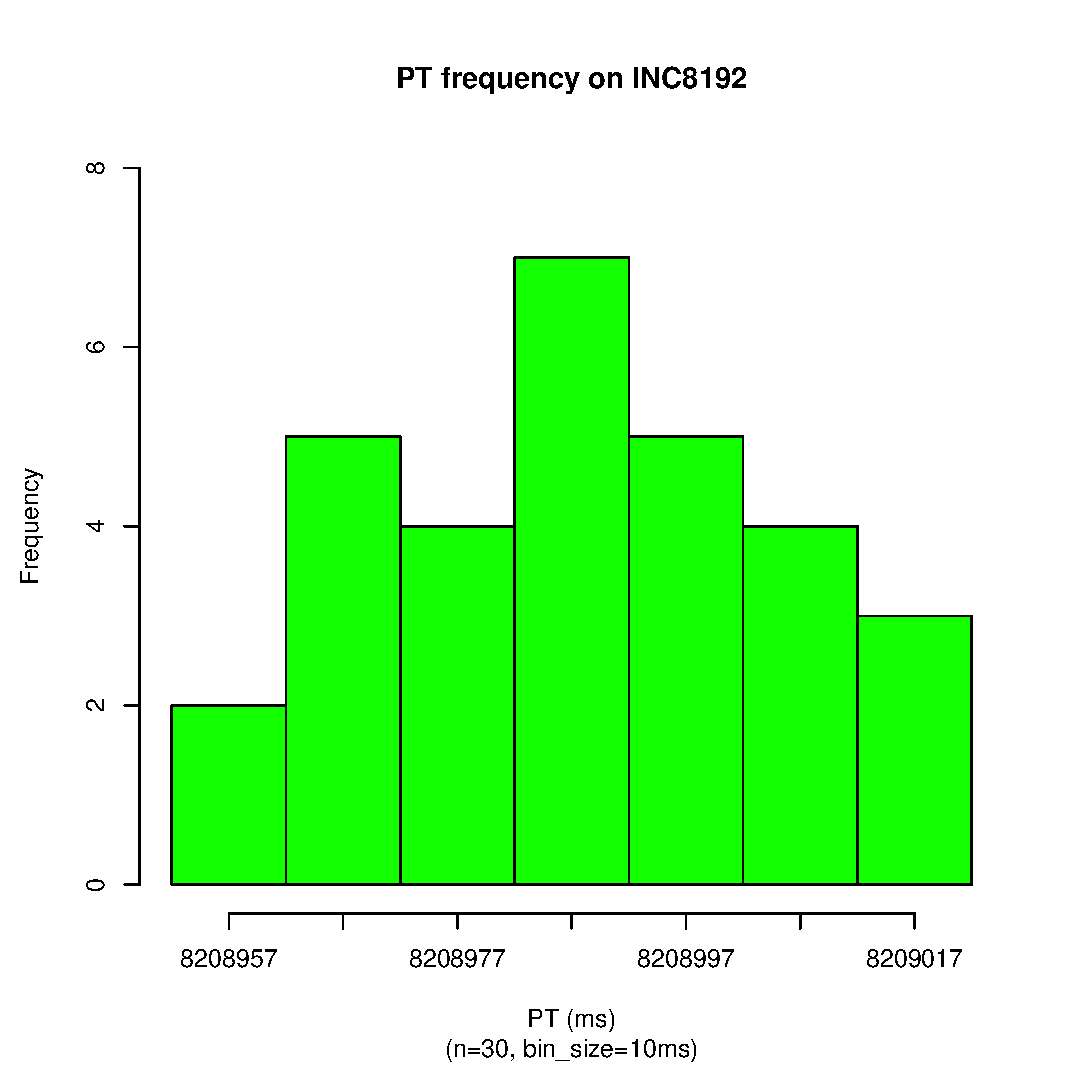
\includegraphics[scale=0.43]{8192_sec_pt_hist.eps}
		\label{fig:inc8192}
	}
	\subfigure[PT frequency on INC16384 on {\tt sodb12}]{
		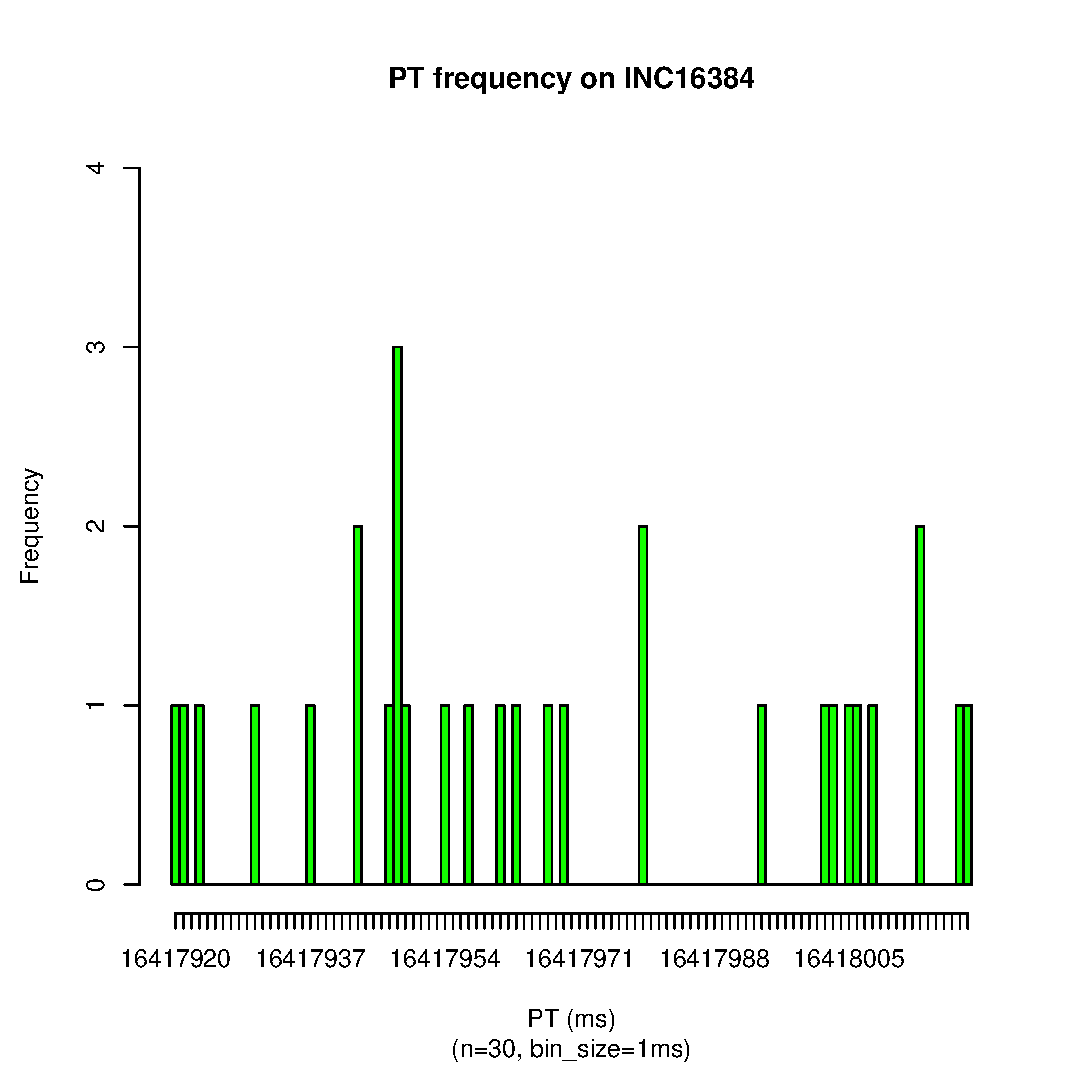
\includegraphics[scale=0.43]{16384_sec_pt_hist.eps}
		\label{fig:inc16384}
	}
	\caption{PT Histograms of INC2048 ... INC16384~\label{fig:s9_r2_pt_hist4}}
\end{figure}

\newpage
\section{Decomposition of INC16 Samples}

\begin{figure}[hp!]
	\centering
	\subfigure[PT frequency on INC16 with the first 200 samples on {\tt sodb9}]{
		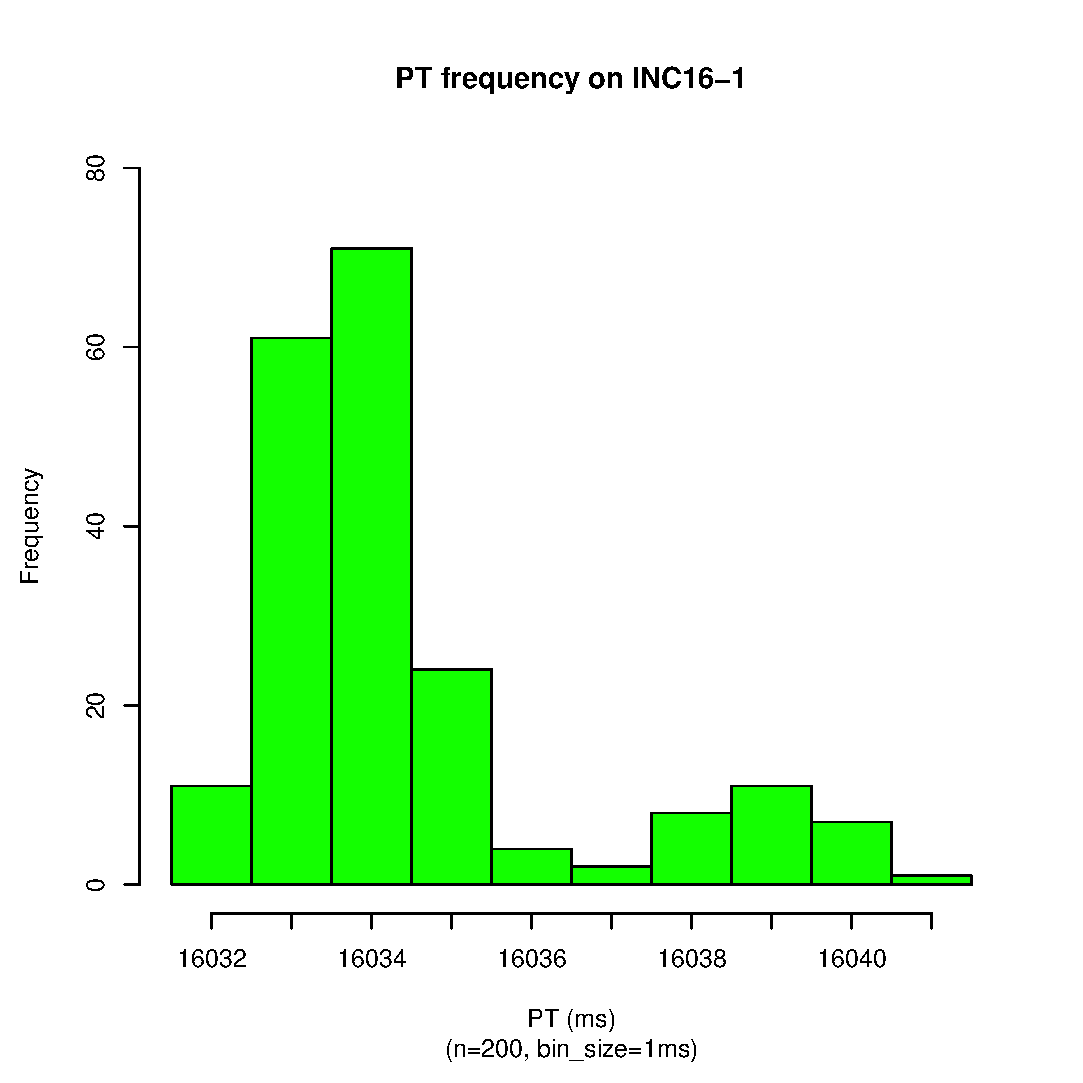
\includegraphics[scale=0.43]{16_sec_pt_hist0_1.eps}
		\label{fig:inc16-1}
	}
	\subfigure[PT frequency on INC16 with the next 200 samples on {\tt sodb9}]{
		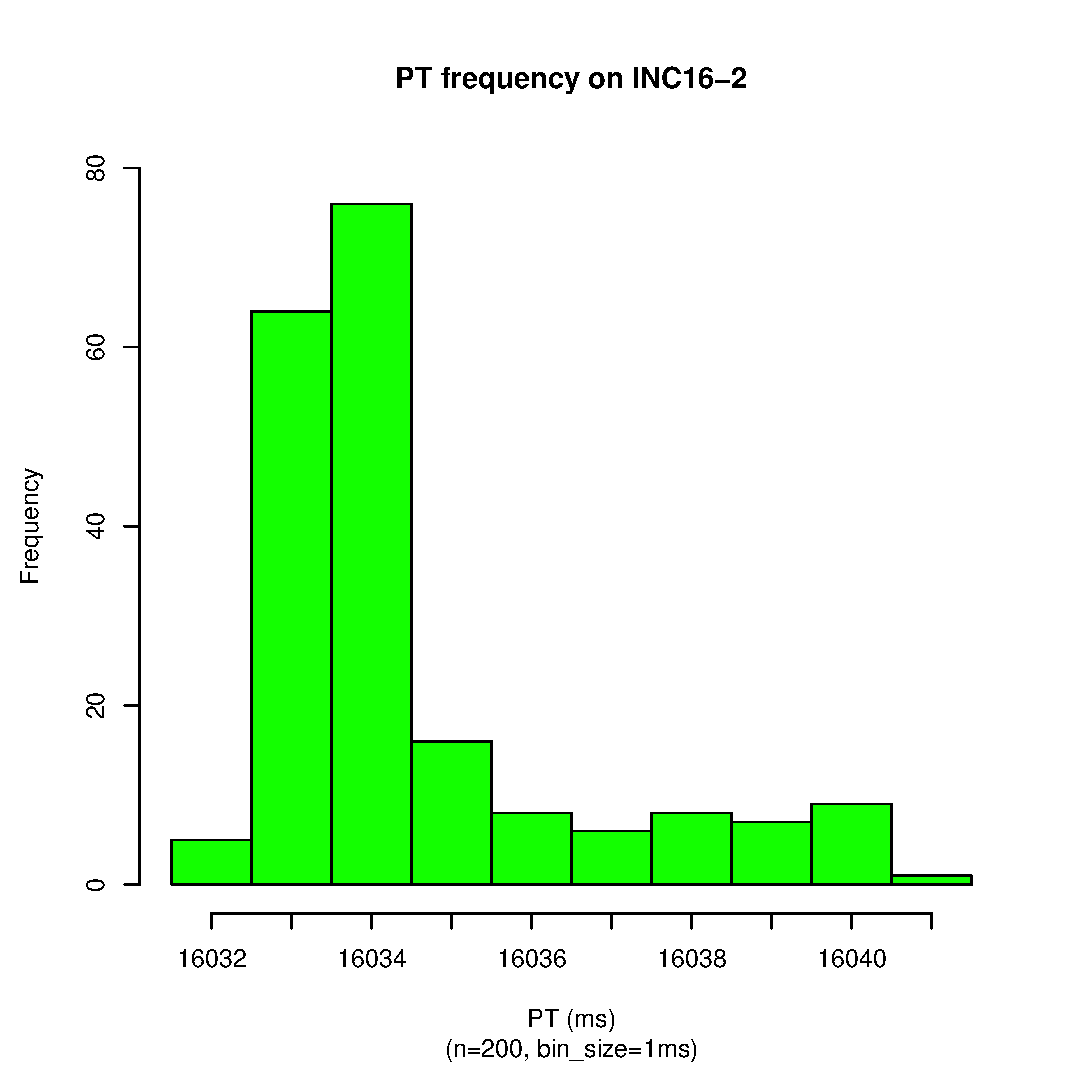
\includegraphics[scale=0.43]{16_sec_pt_hist0_2.eps}
		\label{fig:inc16-2}
	}
	\subfigure[PT frequency on INC16 with the next 200 samples on {\tt sodb9}]{
		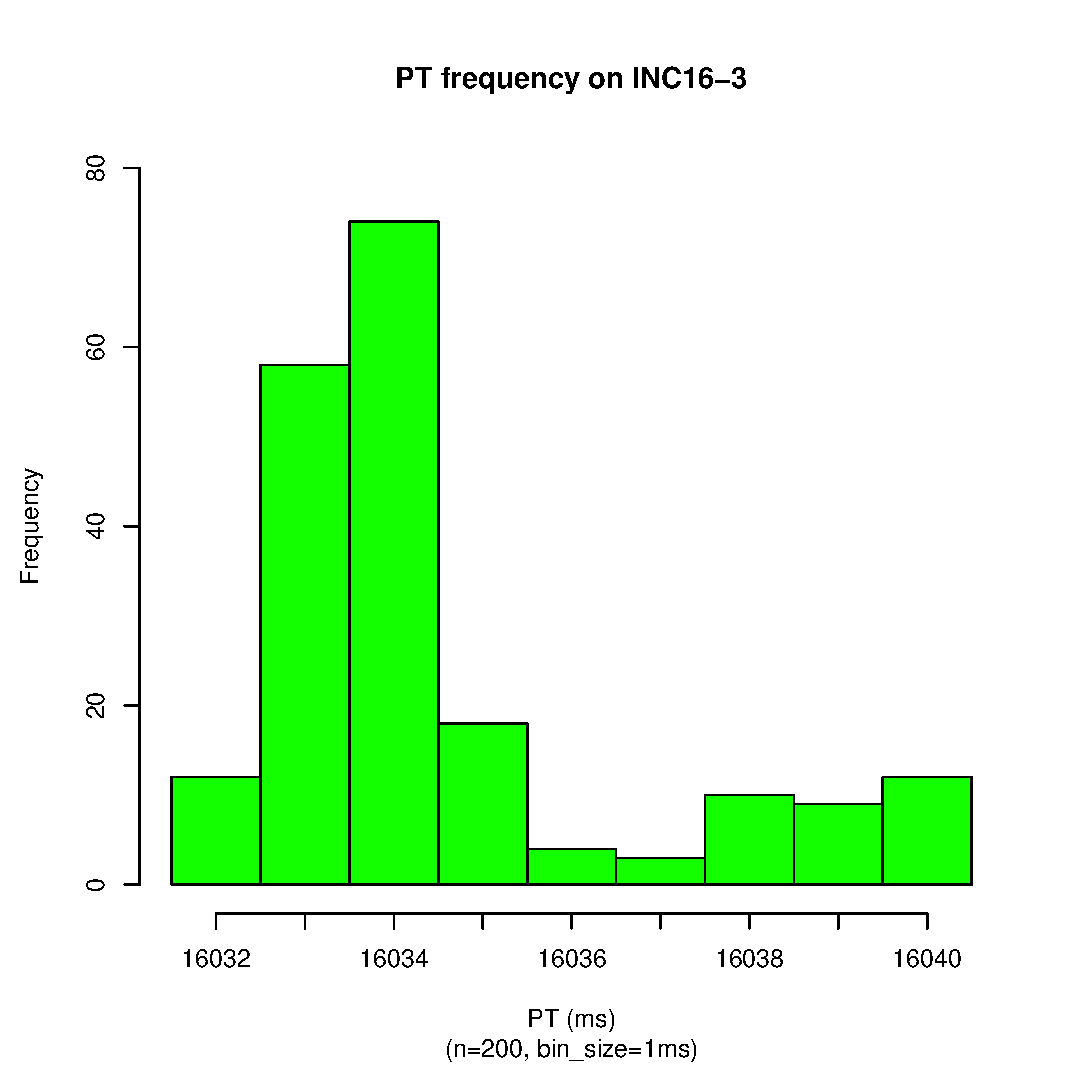
\includegraphics[scale=0.43]{16_sec_pt_hist0_3.eps}
		\label{fig:inc16-3}
	}
	\caption{PT Histograms of INC16-1 ~ INC16-3~\label{fig:inc16_hist1}}
\end{figure}

\begin{figure}[hp!]
	\centering
	\subfigure[PT frequency on INC16 with the next 200 samples on {\tt sodb9}]{
		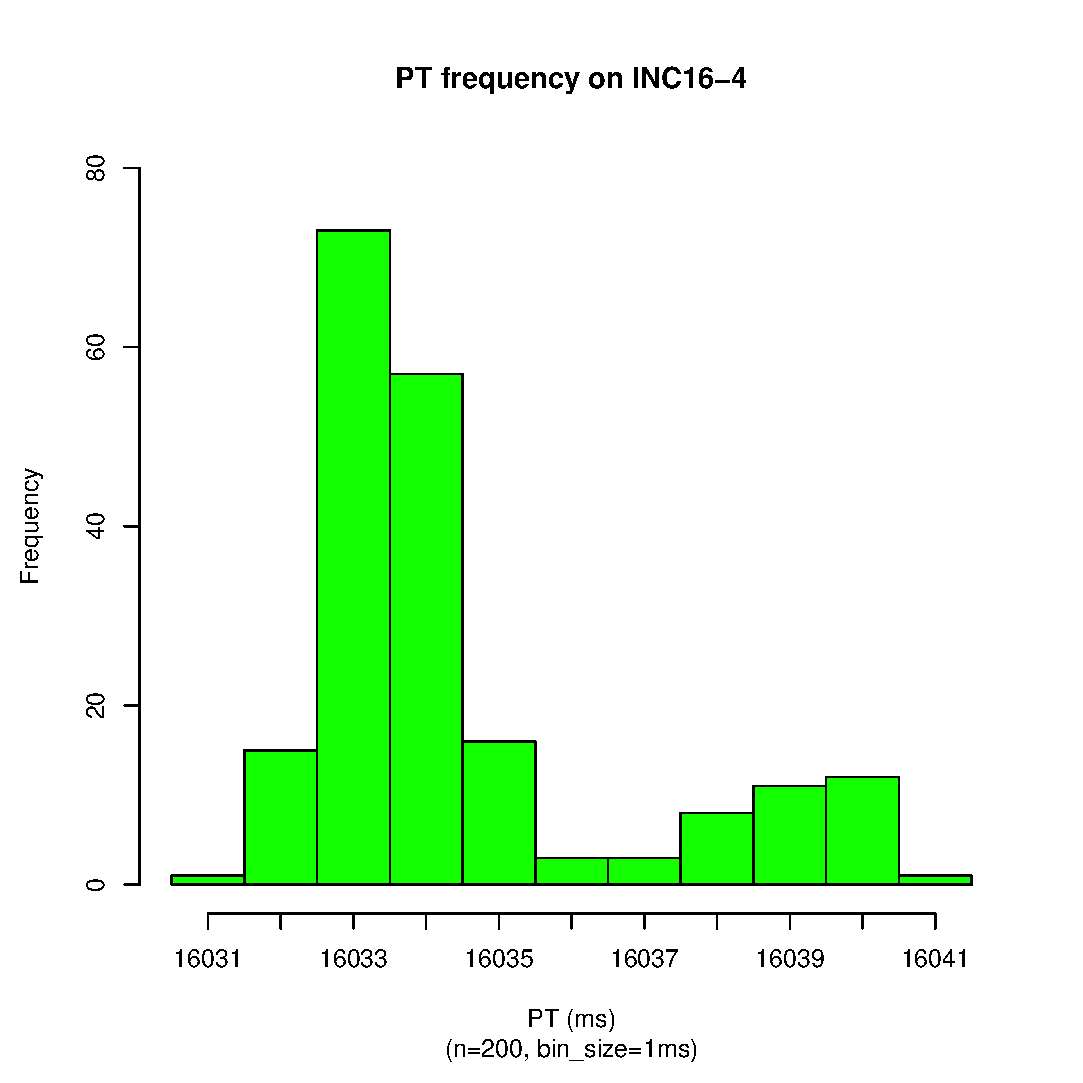
\includegraphics[scale=0.43]{16_sec_pt_hist0_4.eps}
		\label{fig:inc16-4}
	}
	\subfigure[PT frequency on INC16 with the next 200 samples on {\tt sodb9}]{
		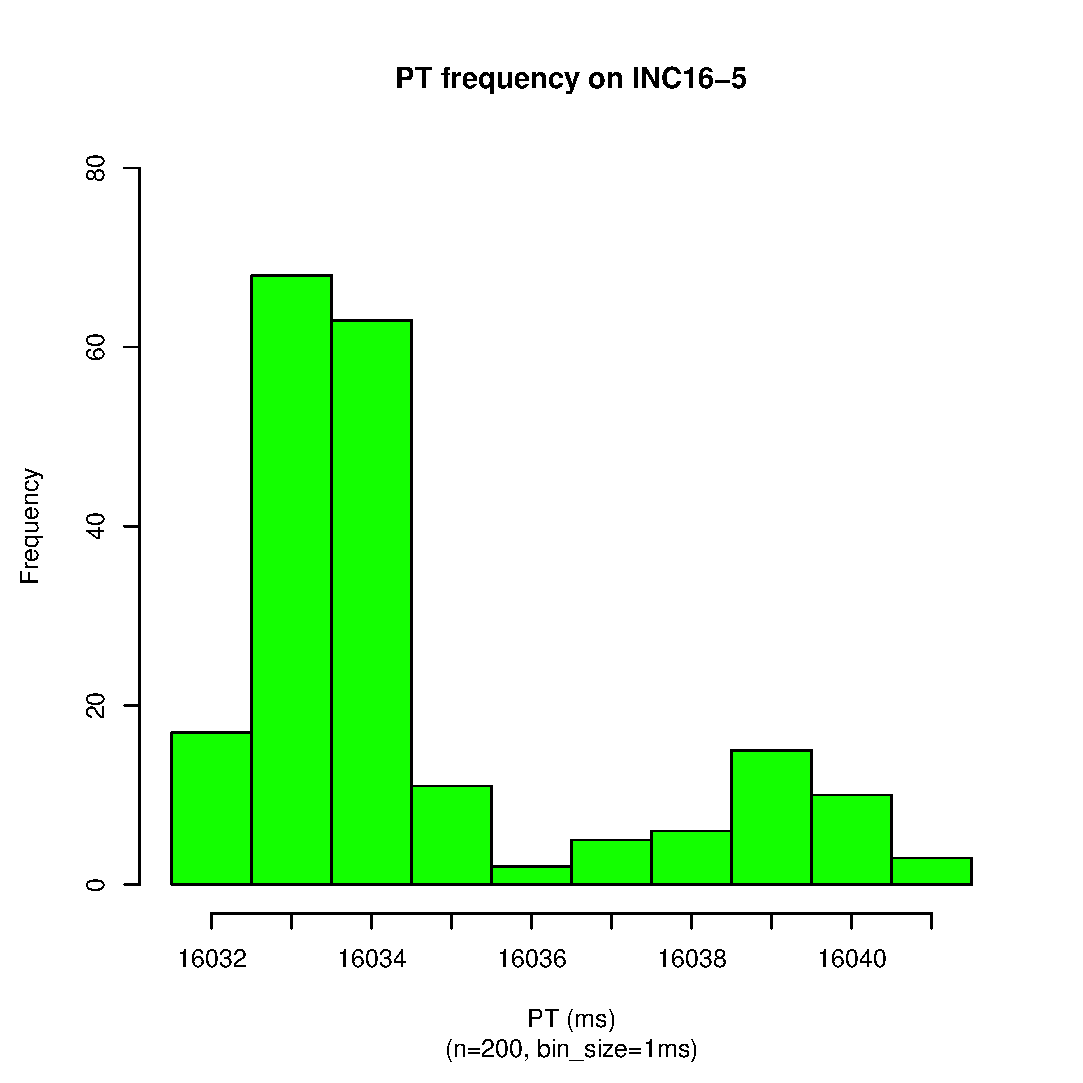
\includegraphics[scale=0.43]{16_sec_pt_hist0_5.eps}
		\label{fig:inc16-5}
	}
	\caption{PT Histograms of INC16-4 ~ INC16-5\label{fig:inc16_hist2}}
\end{figure}

\end{document}